%  \documentclass[10pt]{article}
% %\usepackage[margin=.4in]{geometry} 
% \usepackage[left=.25in,top=.25in,right=.25in,head=.3in,foot=.3in]{geometry}
% \usepackage[pdftex]{graphicx} 
% \usepackage{epstopdf}  
% \usepackage{verbatim}
% \usepackage{amssymb} 
% \usepackage{setspace}   
% \usepackage{longtale}  

% \newenvironment{cin}[1]{
% \begin{center}
%  \input{#1}  

% \end{center}}


% \usepackage{natbib}
% \bibpunct{(}{)}{,}{a}{,}{,}


%on *part1_set_up
\documentclass[11pt]{article}      
\usepackage[margin=10pt,font=small,labelfont=bf]{caption}[2007/03/09]

%\long\def\symbolfootnote[#1]#2{\begingroup% 							%these can be used to make footnote  nonnumeric asterick, dagger etc
%\def\thefootnote{\fnsymbol{footnote}}\footnote[#1]{#2}\endgroup}		%see: http://help-csli.stanford.edu/tex/latex-footnotes.shtml
%%
%#  \abovecaptionskip: space above caption
%# \belowcaptionskip: space below caption
%%
% %
\usepackage{setspace}
\usepackage{longtable}
%\usepackage{natbib}
\usepackage{anysize}
% %
\usepackage{natbib}
\bibpunct{(}{)}{,}{a}{,}{,}

\usepackage{amsmath} % Typical maths resource packages
\usepackage[pdftex]{graphicx}                 % Packages to allow inclusion of graphics
%\usepackage{color}					% For creating coloured text and background
\usepackage{epstopdf}
\usepackage{hyperref}                 % For creating hyperlinks in cross references
\usepackage{color}


% \hypersetup{
%     colorlinks = true,
%     linkcolor = red,
%     anchorcolor = red,
%     citecolor = blue,
%     filecolor = red,
%     pagecolor = red,
%     urlcolor = red
% }


% \newenvironment{rr}[1]{
% \hspace{-1in}
% \texttt{[{#1}]} 
% \hspace{.1in}}
% \newenvironment{rr}[1]{
% % \hspace{-.475in}
% % $>>>$
% }

\usepackage{changepage}   % for the adjustwidth environment
\newenvironment{cc}[1]{ 
\begin{adjustwidth}{-1.5cm}{}
  \vspace{.3 in}
  {\color{blue} \footnotesize  {#1}}
  \vspace{.1in}
\end{adjustwidth}
}






%\oddsidemargin 0cm
%\evensidemargin 0cm
%\pagestyle{myheadings}         % Option to put page headers
                               % Needed \documentclass[a4paper,twoside]{article}
%\markboth{{\small\it Politics and Life Satisfaction }}
%{{\small\it Adam Okulicz-Kozaryn} }
\marginsize{2cm}{2cm}{0cm}{1cm} %\marginsize{left}{right}{top}{bottom}:
\renewcommand\familydefault{\sfdefault}
%\headsep 1.5cm

% \pagestyle{empty}			% no page numbers
% \parindent  15.mm			% indent paragraph by this much
% \parskip     2.mm			% space between paragraphs
% \mathindent 20.mm			% indent matheistequations by this much

					% Helps LaTeX put figures where YOU want
 \renewcommand{\topfraction}{.9}	% 90% of page top can be a float
 \renewcommand{\bottomfraction}{.9}	% 90% of page bottom can be a float
 \renewcommand{\textfraction}{0.1}	% only 10% of page must to be text

% no section number display
%\makeatletter
%\def\@seccntformat#1{}
%\makeatother
% no numbers in toc
%\renewcommand{\numberline}[1]{}
 
\newenvironment{ig}[1]{
\begin{center}
 %\includegraphics[height=5.0in]{#1} 
 \includegraphics[height=3.3in]{#1} 
\end{center}}

\usepackage{pdfpages}

%this disables indenting--looks cleraner that way
\newlength\tindent
\setlength{\tindent}{\parindent}
\setlength{\parindent}{0pt}
\renewcommand{\indent}{\hspace*{\tindent}}

 
\date{{}\today}
\title{Author's response\\ {\large Manuscript Number: ARIQ-D-23-01167 \\ Title:  The Impact of Covid19 on the Urban-Rural Happiness % Gradient 
  }}

\author{}
%off
%on *part2_intro
\begin{document}
\bibliographystyle{/home/aok/papers/root/tex/ecta}
\maketitle

\tableofcontents

\section{Response to Editor} 


\noindent Dear Professor Burger,\\

\noindent Thank you for the opportunity to submit a revised draft. We have revised the manuscript in light of the reviewers' suggestions. We list below in inline format our brief responses to reviewers' comments and attach at the end tracked changes that show precisely the additions and deletions. In light of the positive peer reviewer's recommendations we are hopeful that you will be able to make a positive decision. We appreciate your consideration. Thank you!\\

%DO NOT SELF IDENTIFY IN THIS BLIND DOCUMENT
\noindent Best,\\
Authors 
\vspace{.5in}

%  \rr{page/paragraph/line} {This is the format of text references}  \hspace{1.5in} 
% \vspace{.2in}


% Let me begin by thanking the anonymous reviewer for helpful
% suggestions. Below, I reply inline to your comments. The
% differences between last submission and this revison follow.

  %  XXXmake here any general remarks if needd e.g. abut use
  % of latex or specific approach/angle  i take in thsi paper that
  % explains why i proceeded in a certian way if reviewer did not see
  % thst--be constructive!!XXX


 
\newpage
\section{Response to Reviewer \#1} 

\cc{I believe the revision has enhanced the paper. However, there is still room
  for improvement.}

thanks

\cc{My specific comments and suggestions follow:

1.      Sample selection and country information:

The paper aims to explore how Covid-19 changed subjective well-being (SWB) in
cities compared to smaller places. For this inquiry the authors select a sample
of countries that can be characterized as severely affected. To what extent the
countries are affected is measured by the number of infected and deaths due to
Covid-19. In my opinion, the paper would benefit from clearly stating this
earlier in the text, explaining the country selection process in detail, and
justifying the decisions made.}


the country selection process fits better in data section; but early on, at the
end of introcuction section we now added:\\

\begin{quote}
  In section ``3 Data'' we focus on the sample selection from World Values
  Surves down to: United Kingdom, the Netherlands, and Uruguay--the countries
  that are severely affected by the pandemic (infections and deaths) and with
  substantial samples available pre/during the pandemic for cities/smaller areas.
\end{quote}

\cc{I believe that the manuscript would be enhanced by additional information on
  the country cases. As there are only three cases, this should be feasible to
  do. What kind of policies/restrictions were implemented during the covid-19
  pandemic? Do the three cases differ in policy responses? Special attention
  should be given to policies that may have had different consequences in cities
  and rural areas. In general, a more detailed description of the country cases
  would improve the paper, assist in interpreting the results (incl. gauging
  external validity), and strengthen the discussion. For instance, when
  interpreting the reduction in SWB for rural areas in GBR (bottom of page 4).}

Note: there was already a section in appendix ``Covid Trends in GBR, NLD, URY''\\

Now added in appendix under ``Variable Definitions and Distributions'' crosstabs by country and urbanicity and wave\\

And to your point, in terms of policy responses, we have found 3 datasources and
added from them in the appendix in a new sec ``Policy Responses in GBR, NLD,
URY''--the information is substantial, but not perfect or complete and while
much information is comparable, there is also a qualitative component not
directly comparable. % we were unable to find more or
% better information\\ 


\cc{The sample consists of both developed countries (GBR and NLD) and a
  developing country (URY). Does it make sense to pool data from countries at
  different stages of development? Are developing and developed countries
  expected to be affected by Covid-19 in a similar fashion? Including more
  justification regarding this decision would improve the manuscript.}

We name in the abstract the three countries studied.\\ %was already there

Now, also to better orient the reader re sample selection early on, we added at
the end of introduction:\\

\begin{quote}
  In section ``3 Data'' we focus on the sample selection from World Values
  Surves down to: United Kingdom, the Netherlands, and Uruguay--the countries
  that are severely affected by the pandemic (infections and deaths) and with
  substantial samples available pre/during the pandemic for cities/smaller areas.
\end{quote}

Yes! agreed, the countries are diverse! And this is the very reason  we first
proceed country-by-country, and only then introduce a pooled model--we now add
this point in a footnote in the ms. And note, in the pooled model, as countries
are quite diverse, we had country dummies--this point is also now made in the
manuscript. 

\cc{The authors begin the abstract by referring to "the developed world." This
  seems somewhat unsatisfactory given that the paper also uses data from a
  developing country. In my opinion, it would also be beneficial to add text and
  references on urban-rural happiness in developing countries, or perhaps focus
  more on sources of happiness in different places (se under bullet point 4 for
  elaboration).}

We meant th egeneral background info on the urban-rural happiness gradient more
pronunced in the developed countries. But, yes, a fair point, it might have been
confusing--now dropped "the developed world'' from abstract.\\

\cc{2.      Tables:

I am not convinced by the argument made for not having Table 6 in the main text
of the paper. The text related to tables 1-3 is focused on comparing what
happens in places of different population sizes. The reader will be interested
in seeing if these differences are statistically significant.}

With 2 figures and 4 tables, it's already plenty of displays, a total of 6; our
philosophy was to focus on main findings in the paper and postpone auxiliary
analyses to appendix like done in top outlets such as Nature, Science, or
PNAS.\\

Another reason is that it's not just adding table 6--there is a closely related
crosstab table following it and another table with alternative specification; hence it would be adding 3 tables, not one.

Still, you have a point ``The reader will be interested
in seeing if these differences are statistically significant''

Therefore there is the following text following table 3 in the body of the ms:
% was already there duh

\begin{quote}
  In the online appendix we do not split by urban/rural but instead we add a urban/rural dummy and interaction with the
pandemic dummy--the interaction is statistically insignificant, i.e., the pandemic differential urban v rural effect is not
statistically significant if split by country. However, if the urbanicity variable is not collapsed into the binary urban-rural,
but left as several categories, the differences for the Great Britain and Uruguay are statistically significant.
\end{quote}

\cc{3.      Significance levels:

It would be helpful to have some more information on the uncertainty of the
estimates. Can you add the estimated standard errors to the OLS tables, or at
least provide a description of the significance levels indicated by the stars in
a table footer?}

yes, apologies, formatting issue in word, now submitted as LaTeX with
significance levels in footer

\cc{4.      Interpretation of "the effect":

The statement "There is a direction, it's just not causal" is very
confusing. With the research design used, it would be hard to defend these as
causal estimates. For instance, one potential threat to identification is that
slower diffusion of infectious disease to rural areas compared to urban areas
may have affected the results (in line with the reference in the manuscript by
Cuadros et al. 2021). Another threat, which the authors also mention, is omitted
variables. Perhaps it is better to call these estimates associations or
relationships?}

we added a a paragraph in limitations sec highlighting your points

we do not say in ms ``There is a direction, it's just not causal''\\

we say in abs:
\begin{quote}
  As in any
 non-experimental research, causality may not be present.
\end{quote}

``Perhaps it is better to call these estimates associations or
relationships?''--again we do highlight aleady in abs that data are
non-experimental and hence causality may not be present; still, the results are more than associations--we control for predictors of DV; we conduct robustness checks
 with different sepcifications, and have before-after (pre and during pandemic)
 2 group (urban rural) specification, so called difference-in-difference
 (DID).--we highlight these points in the added paragraph as well.

\cc{I am also curious about how the authors interpret the impact of Covid-19. Is
  it narrowly focused on disease and mortality (and the scare inflicted by such
  happenings to people in the vicinity), or could economic consequences of
  restrictions, such as unemployment, also be part of the relationship? There
  are potentially many sources to life satisfaction in both rural and urban
  areas. One of the standard arguments for urban advantage is the availability
  of commodities, services, and work/career opportunities. The opportunity to
  take advantage of such amenities were perhaps also reduced by the
  restrictions? I think the paper could benefit from elaborating on such a
  "bundle view/domain satisfaction view" of life satisfaction. Such a
  perspective is indirectly mentioned with exposure to nature being defined as a
  rural amenity (first paragraph of Section 2), and the faster spread of
  infectious disease being an urban disamenity.}
  
%yes not just covid but its conssequences notably as we say distancing  in itself etc\\

yes totally! it is arguably also reduction in urban amenities availibility! we
have hinted at it earlier but now elaborate in discussion section--thank you!
%maybe where i have soc dist in itself

\cc{Other comments:

  Table 2 and 3 have the same heading.}

fixed (in fact all tables 1-3 had the same heading)

\cc{As mentioned by reviewer 2, you do not investigate what happens post
  Covid-19. The first part of the introduction would benefit from reflecting
  this.}

we have fixed that already earlier: it is pre v during; not post\\
also reviewer 2 says she has  been satisfied with the revison

\cc{The conclusion and discussion section references the US case quite
  frequently. It would benefit from focusing more on the countries studied. I do
  not see the relevance of the last paragraph in this section.}

Much data and research on the topic is from the US. Both of us live in the US
and have an understanding of urbanization, happines, and covid in the US.\\

Still, we cut on the US where it was less relevant.\\

We have rephrazed the last paragraph so it is better connected to the article.\\

\cc{I can imagine that surveys were hard to collect in the countries were Covid-19 hit hardest. Perhaps include some reflections on this and how it might have affected the results? Did it change the response rates?}

one would imagine, still the samples are quite large during the pandemic across
the urbanicity--see crosstabs in appendix\\

\cc{Limitations and future research: You talk about generalization and countries with different covid-19 infection rates. This is something you have started to look at in the appendix - by including some simple analysis of Marocco and Venezuela. These examples can perhaps be used more actively in the discussion section? In the appendix, perhaps add similar regressions of these countries as the others?}

Marocco and Venezuela are very special cases as explained in data section,
that's why they are postponed to appendix, these are auxiliary only


\newpage
\section{Response to Reviewer \#2} 

\cc{You have done a good job revising your manuscript. You have satisfactorily responded to all my remarks and suggestions.}

great! thanks!

\cc{My comments are now minor and concern various errors/omissions in the reference list:

- You do not cite the two publications by Carlsen and Leknes correctly/fully in the reference list. With regards to the first, you write "unpublished" and year 2019, and with regards to the second, you write Regional Studies without informing about the volume number and the page numbers. The correct citations are:

Carlsen, F., and Leknes, S. (2022a). The paradox of the unhappy, growing city: Reconciling evidence. Cities, 126, 103648.

Carlsen, F., and Leknes, S. (2022b). For whom are cities good places to live? Regional Studies, 56(12), 2177-2190.

And consequently, on page 2, line 15/16, instead of "Carlsen and Leknes (2019, 2022)", please write "Carlsen and Leknes (2022a, 2022b)".

- On page 2, line 14, you write "Sorensen (2020)", but the surname is spelled wrong, and the publication year is wrong. So instead of "Sorensen (2020)", please write "Sørensen (2021)". In the citation in the reference list, the surname and the publication year are also wrong. In addition, the citation lacks both the volume number and the article number. The correct citation to write in the reference list is the following:

Sørensen, J. F. L. (2021). The rural happiness paradox in developed countries. Social Science Research, 98, 102581.}

done; note the bib style used displays only volume wothout number so its 56; not
56(12); if the journal requires number as well, it will be added in
publishing/proofreading stage


\newpage
\bibliography{/home/aok/papers/root/tex/ebib}

\section{Tracked Text Changes}  
\textbf{(see next page)}

% use ediff to pull the latest revison and just save it as rev0
% or better: git show f370f9881d0dd450b2f6856824b3058e421da6bc:micah_eu_lr_welf.tex >/tmp/a.tex 
% (original state that was submitted) and then just:
% latexdiff old.tex new.tex > old-new.tex
% pdflatex diff.tex [if want bib open in emacs and do usual latex/bibtex]
% and then 
% gs -dBATCH -dNOPAUSE -q -sDEVICE=pdfwrite -sOutputFile=respnseAndTrackedChanges.pdf rev.pdf diff.pdf 
% this aint working:(
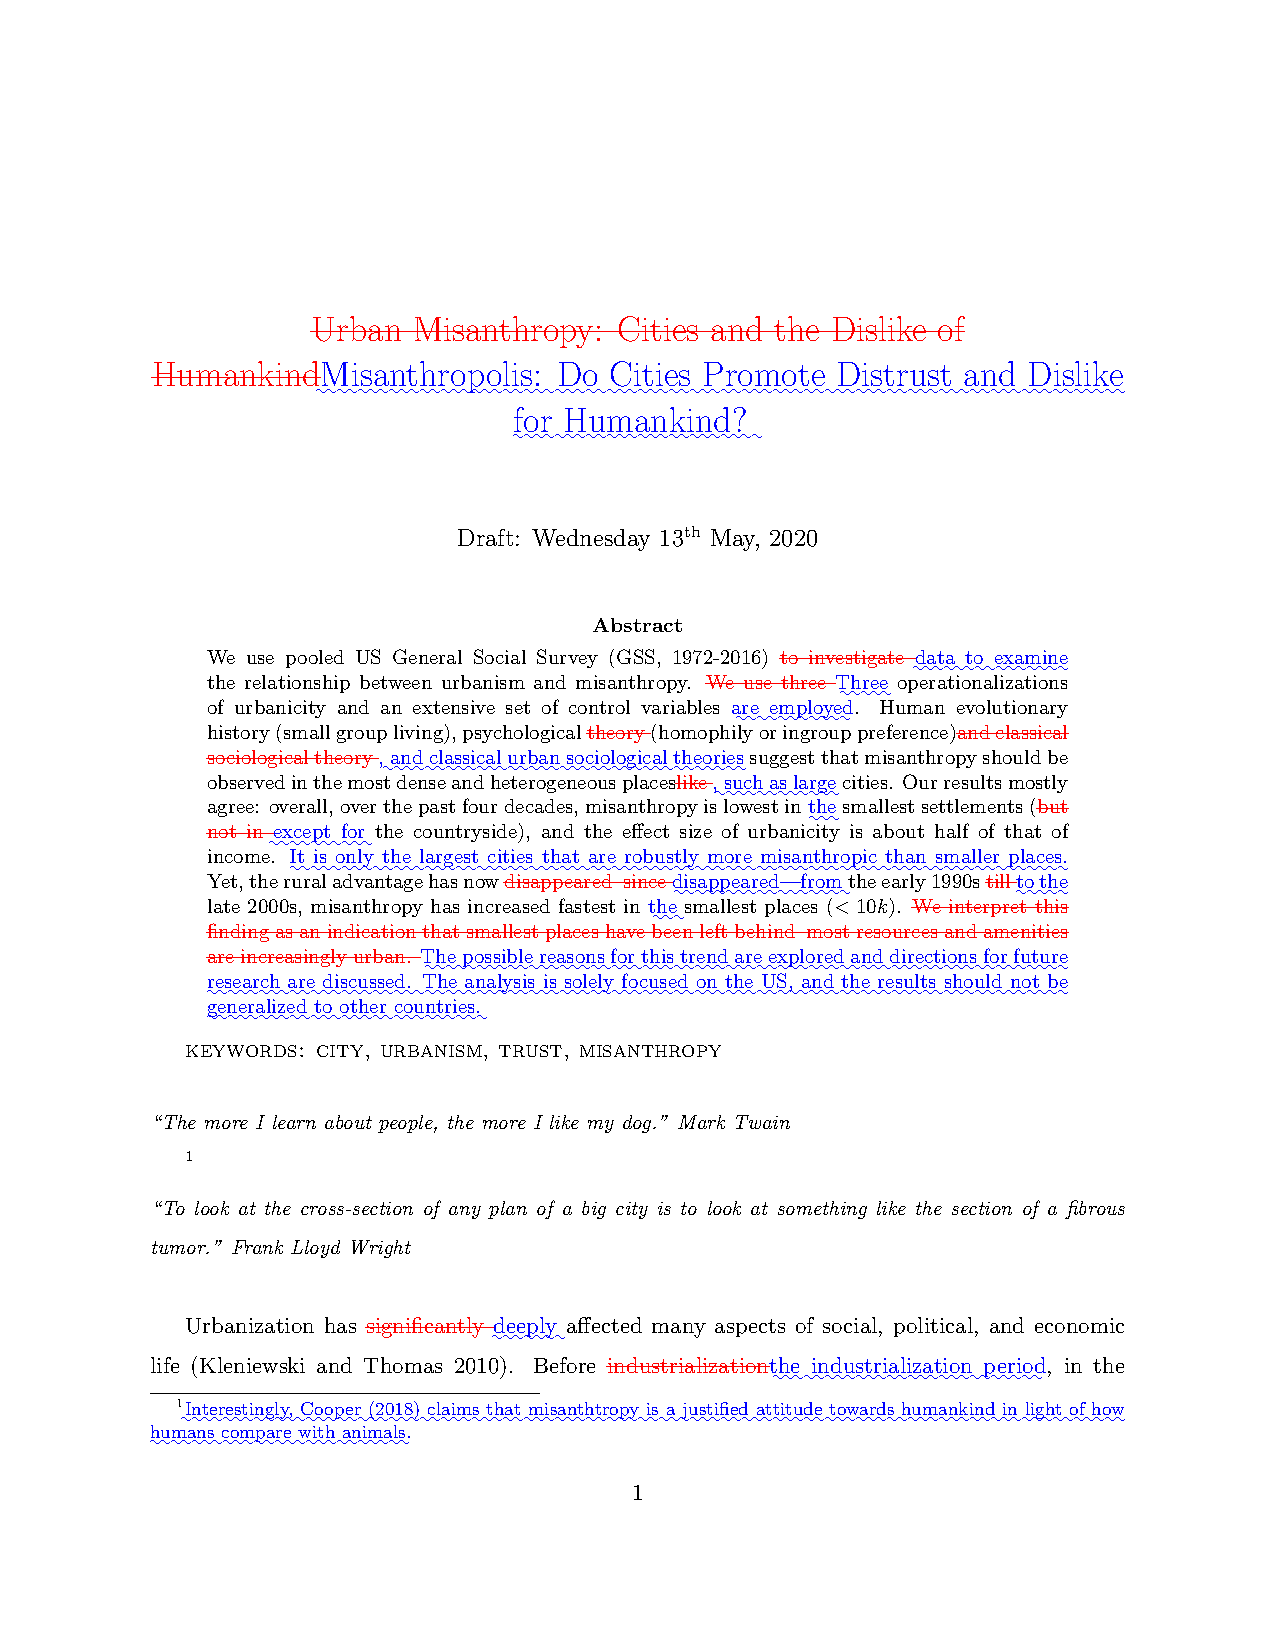
\includepdf[pages={-}]{old-new2.pdf}%don't forget to latex diff.tex!

\end{document}
%off

Added:
\begin{quote}
\input{/tmp/a1}
\end{quote}

%make sure that tags are in newline and at the begiiing!!!

sed -n '/%a1/,/%a1/p' /home/aok/papers/root/rr/ruut_inc_ine/tex/ruut_inc_ine.tex | sed '/^%a1/d' > /tmp/a1

sed -n '/%a2/,/%a2/p' /home/aok/papers/root/rr/ruut_inc_ine/tex/ruut_inc_ine.tex | sed '/^%a2/d' > /tmp/a2

sed -n '/%a3/,/%a3/p' /home/aok/papers/root/rr/ruut_inc_ine/tex/ruut_inc_ine.tex | sed '/^%a3/d' > /tmp/a3

sed -n '/%a4/,/%a4/p' /home/aok/papers/root/rr/ruut_inc_ine/tex/ruut_inc_ine.tex | sed '/^%a4/d' > /tmp/a4

sed -n '/%a5/,/%a5/p' /home/aok/papers/root/rr/ruut_inc_ine/tex/ruut_inc_ine.tex | sed '/^%a5/d' > /tmp/a5

sed -n '/%a6/,/%a6/p' /home/aok/papers/root/rr/ls_fischer/tex/ls_fischer.tex | sed '/^%a6/d' > /tmp/a6

sed -n '/%a7/,/%a7/p' /home/aok/papers/root/rr/ls_fischer/tex/ls_fischer.tex | sed '/^%a7/d' > /tmp/a7

sed -n '/%a8/,/%a8/p' /home/aok/papers/root/rr/ls_fischer/tex/ls_fischer.tex | sed '/^%a8/d' > /tmp/a8

sed -n '/%a9/,/%a9/p' /home/aok/papers/root/rr/ls_fischer/tex/ls_fischer.tex | sed '/^%a9/d' > /tmp/a9

#note has to be 010! otherwhise it picks a1!
sed -n '/%a010/,/%a010/p' /home/aok/papers/root/rr/ls_fischer/tex/ls_fischer.tex | sed '/^%a010/d' > /tmp/a010















\section*{Response to Reviewer \#2} 
\cc{In recent years an interest has developed in comparing quality of life on both sides of the Atlantic. This paper gives a refreshingly crisp report on why are there such marked differences in satisfaction with working hours in the US and Europe, a topic that according to the author is underrepresented in the QOL literature. The author pits cultural against economic reasons to explain preferences for longer and shorter working hours. An excursion into the value attached to work in the two study contexts suggests an explanation (see Table 2 and Figure 3). A major strength is the care taken to harmonise relevant data collected on both sides of the Atlantic.}

\rr{n/a} N/A

\cc{Quibbles:\\
Tables and graphs in the text are kept to a minimum. The remainder of the evidence is placed in the
appendices. This seems to work well.}

\rr{n/a} N/A


\cc {However, readers might like to see the questions contained in Tables 8 and 9 repeated in the
  legends to Tables 9 - 16, and Tables 18-20.} 

\rr{10-19//}  To make the appendices more concise I decreased spacing in tables from
1.5 to 1.0. As a result, there are now on average 3 tables per page instead of 2, and it is easier to
find them. Also length of the
manuscript decreased from  26 to 22 pages, which  saves space in the journal. Repeating questions in
legends will take up space and not clarify much: frequency tables are fairly self-explanatory.

\cc{The alignment of several items in Table 8 is incorrect and the wording of the item on the showcard for 'GSS friends' is missing: say: 'How often do you see your friends?'}

\rr{13//}  I fixed the alignment in Table 8 in column 1. And added ``Spend a social evening with friends who live outside the neighborhood?''


\section*{Reviewer \#3}

\cc{ This paper intends to explain the difference between Europeans and Americans
on work and happiness. It finds that Europeans work to live and Americans live to work. This is
indeed a cultural explanation which deserves attention of the academic field in the study of
subjective wellbeing.}

\rr{n/a} N/A

\cc{ In my view, the litmus test of this paper for acceptance of publication is
whether it uses the same measure of subjective wellbeing; as life satisfaction and happiness are
different, despite both are subjective wellbeing. The paper recognizes this difference and clearly
illustrates it in footnote no. 3, but it makes it clear that they are used interchangeably. This is
fine if two concepts are the same; however, when we go to the measurement -the Europeans were asked
about the extent of satisfaction "with the life you (respondents) lead"; so, this is a life
satisfaction measure. To the Americans, the question they were asked is the extent of happiness of
"things are these days";
so, this is a happiness measure. Therefore, the Europeans were asked about a cognitive judgment of
their life; a long period of time up to the moment they were interviewed. But Americans were asked
differently - "things are these days" indicates a shorter span of time and the idea is only about an
affective mood - happiness, without any cognitive evaluation as in the case of life satisfaction. In
other words, both concepts should not be treated as the same on the operational level in this
paper.}

\rr{5/2/6} This wording difference was acknowledged in the paper:

\begin{quote}
 Wording of the
survey questions is slightly
different (see  Appendix B), but these small
differences do not make surveys
incomparable. At least one other paper used the same surveys
to conduct successful comparisons
between Europe and the US (see \citet{alesina03}). 
\end{quote}

\noindent\citet[2013/2/11]{alesina03} defended this approach arguing that:
\begin{quote}
 ``happiness'' and ``life satisfaction'' are
highly correlated. 
\end{quote}


\noindent I reviewed recent literature and found another published paper  using the same survey items. \citet[211/2/20]{stevenson09w} defend this approach arguing that:  
\begin{quote}
While life satisfaction and happiness are somewhat different
concepts, responses are highly correlated.
\end{quote}

\noindent \citet{alesina03} \citet{stevenson09w} are able to make statements about correlations and compare
happiness with life satisfaction because there was happiness question in addition to life
satisfaction question in Eurobarometer until 1986
(still, they use life satisfaction measure because it is available for more years).
I use Eurobarometers in 1998 and 2001 (these are the only datasets with working hours available
for Europe) and I have to use ``life satisfaction'' measure. Both, \citet{alesina03} and
\citet{stevenson09w} use \underline{exactly the same survey items as this paper uses} to compare
happiness in the U.S. and Europe.

\rr{5/2/6} I have changed text FROM:

\begin{quote}
 Wording of the
survey questions is slightly
different (see  Appendix B), but these small
differences do not make surveys
incomparable. At least one other paper used the same surveys
to conduct successful comparisons
between Europe and the US (see \citet{alesina03}). 
\end{quote}

\noindent TO:

\begin{quote}
Wording of the
survey questions is slightly
different (see  Appendix B), but these small
differences do not make surveys
incomparable. At least two other papers used the same surveys
to conduct successful comparisons
between Europe and the US (see \citet{alesina03, stevenson09w}). ``Happiness'' and ``Life
Satisfaction'' measures are highly correlated. 
\end{quote}

\noindent Still, using different measures may be a limitation of this study, and this pertains to
independent variables as well. This limitation is acknowledged by adding  
footnote 5 on p. 5.

\begin{quote}
 Still, robustness of the results can be improved if wording of the survey
 questions is the same for all respondents. This remains for the future research when better data
 become available.
\end{quote}


\cc{Of course, a composite index combining both happiness and life satisfaction is a solution;
but unfortunately, this paper does not have it for this comparative study on subjective wellbeing
between Europeans and Americans. On the basis of this assessment, I do not recommend to accept the
paper for publication in its present form.}

\rr{n/a} If I understand this comment correctly, reviewer asks to combine happiness for the
U.S. with life satisfaction for Europe, but I believe this to be a misunderstanding: In order to
combine two different  measures into an index they need to be observed for the same
 individuals. This is not the case here: there is happiness for Americans and life satisfaction for Europeans.

\noindent The only way to create an index is to find both happiness and life satisfaction measures in the same
dataset, but they do not
exist. Again, this is not a serious limitation because happiness and life satisfaction
are highly correlated and the very same measures as used in this paper are successfully used in the
literature  \citep{alesina03, stevenson09w}.

